\documentclass{article}
\setlength{\oddsidemargin}{0.25 in}
\setlength{\evensidemargin}{-0.25 in}
\setlength{\topmargin}{-0.6 in}
\setlength{\textwidth}{6.5 in}
\setlength{\textheight}{8.5 in}
\setlength{\headsep}{0.75 in}
\setlength{\parindent}{0 in}
\setlength{\parskip}{0.1 in}

% ===== PACKAGES =====
\usepackage{xcolor, graphicx, wrapfig}
\usepackage{url, hyperref, dirtree, listings}
\usepackage{courier, lipsum}
\usepackage{amsmath,amssymb}
\usepackage{color}
\usepackage{subfigure}
\usepackage{mdframed}
\usepackage{changepage}
\newmdenv[
  topline=false,
  bottomline=false,
  skipabove=\topsep,
  skipbelow=\topsep
]{siderules}
\renewcommand{\abstractname}{}

% ===== NEW COMMAND =====
\definecolor{light-gray}{gray}{0.95}
\newcommand{\code}[1]{\colorbox{light-gray}{\texttt{#1}}}
\lstset{basicstyle=\footnotesize\ttfamily,breaklines=true}

% ===== VARIABLES =====
\def \R{\mathbb{R}}
\def \Pr{\mathbb{P}}
\def \D{{\rm D}}
\def \N{{\rm N}}
\def \xx{{\boldsymbol{\rm x}}}
\def \y{{\rm y}}




% ===== HEADER BOX =====
\newcommand{\lecture}[2]{
\pagestyle{myheadings}
\thispagestyle{plain}
\newpage
\noindent
\begin{center}
\rule{\textwidth}{1.6pt}\vspace*{-\baselineskip}\vspace*{2pt} % Thick horizontal line
\rule{\textwidth}{0.4pt}\\[1\baselineskip] % Thin horizontal line
\vbox{\vspace{2mm}
\hbox to 6.28in { {\bf CS 760: Machine Learning} \hfill Fall 2020 }
\vspace{4mm}
\hbox to 6.28in { {\Large \hfill #1  \hfill} }
\vspace{4mm}
\hbox to 6.28in { {\scshape Authors:}  #2 \hfill }}
\vspace{-2mm}
\rule{\textwidth}{0.4pt}\vspace*{-\baselineskip}\vspace{3.2pt} % Thin horizontal line
\rule{\textwidth}{1.6pt}\\[\baselineskip] % Thick horizontal line
\end{center}
\vspace*{4mm}
}



% =============== DOCUMENT ===============
\begin{document}
\lecture{Face Mask Detection}{Zijie Zhang}

\begin{center}
{\Large {\sf GO GREEN. AVOID PRINTING, OR PRINT 2-SIDED OR MULTIPAGE.}}
\end{center}

\begin{abstract}
Write your abstract here
\end{abstract}

\section{Introduction}
With the global outbreak of COVID-19, it's even more important to have some policy to mitigate risk. For public safety and health, people are recommended to wear face masks and coverings to control the spread of the COVID-19.

In hospitals and various COVID-19 testing places. If only people wearing masks are allowed to enter, the risk of infection for doctors and staff can be reduced. However, if a potential COVID-19 infected person who is not wearing a mask suddenly appears, there is a high risk of infection in face-to-face communication.

At many intersections, pedestrians will gather briefly while waiting for traffic lights. At this time, the risk of COVID-19 spreading among the population is high. But it is impossible to hire a person to stay at the intersection and remind pedestrians to wear masks.

Similarly, requiring Uber drivers and passengers to wear masks at all times can also effectively reduce the spread of the COVID-19. However, it is impossible to supervise the wearing of masks on moving vehicles in real time.

There are many application scenarios such as this. If it is all supervised by manpower, the investment cost is high, and the health risks of the staff are also high.

Therefore, the need for artificial intelligence to determine the wearing of masks came into being. The main idea of this project is to construct a classifier to judge whether the photo cropped from the face detector is wearing a mask.

\section{Related/Similar work}
% This project is mainly inspired by \textbf{Baidu AI development platform - mask wearing detection products}.

% \url{https://ai.baidu.com/tech/body/driver}


% Related/Similar work:
% \begin{enumerate}
%   \item \url{https://github.com/AIZOOTech/FaceMaskDetection}
%   \item \url{https://github.com/chandrikadeb7/Face-Mask-Detection}
%   \item \url{https://arxiv.org/abs/2003.09093}
% \end{enumerate}

\section{Dataset}



\end{document} 
% This dataset consists of 3835 images belonging to two classes:
% \begin{itemize}
%   \item with\_mask: 1916 images
%   \item without\_mask: 1919 images
% \end{itemize}
% The images used were real images of faces wearing masks. The images were collected from the following sources:
% \begin{enumerate}
%   \item \url{https://github.com/chandrikadeb7/Face-Mask-Detection}
%   \item RMFD dataset(\url{https://github.com/X-zhangyang/Real-World-Masked-Face-Dataset})
%   \item MAFA dataset(\url{https://www.kaggle.com/rahulmangalampalli/mafa-data})
% \end{enumerate}
% The following is the directory structure:
% \DTsetlength{0.2em}{1em}{0.2em}{1pt}{3pt}
%   \dirtree{%
%   .1 .
%   .2 dataset.
%   .3 with\_mask \ldots{} \begin{minipage}[t]{5cm}
%     1916 images{.}
%     \end{minipage}.
%   .3 without\_mask \ldots{} \begin{minipage}[t]{5cm}
%     1919 images{.}
%     \end{minipage}.
%   }

% \section{Approach}

% \subsection{Preprocessing}
% \begin{itemize}
%   \item \code{data\_dir = "../dataset"}\\
%         \code{PATH = list(paths.list\_images(data\_dir))}
%   \item Load images:\\
%         The RGB channel values are in the [0, 255] range. We don’t need all the information of the three color channels, just convert the image to grayscale.
%   \item Rescale all images to the same size.\\
%         \code{image = cv2.imread(img\_path, 0)}\\
%         \code{image = cv2.resize(image, (img\_width, img\_height))}
%   \item Standardize data:\\
%         \code{image = image.flatten()/255.0}
% \end{itemize}

% So far, every image has been transformed into a vector with a length of 50176.
% This will make it more convenient to use PCA to extract the principal components.

% \subsection{Visualize the data}
% \begin{center}
%   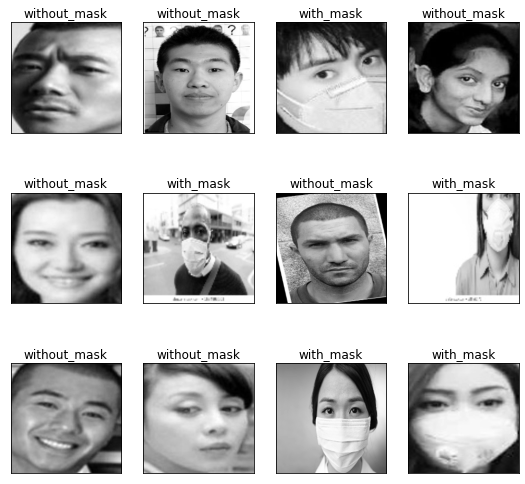
\includegraphics[width=10cm]{preview1.png}
% \end{center}

% \subsection{Data augmentation}
% Due to the small number of training samples in this data set, overfitting generally occurs. Data augmentation takes the approach of generating additional training data from existing examples by augmenting them using random transformations that yield believable-looking images. This helps expose the model to more aspects of the data and generalize better.\\
% \begin{center}
%   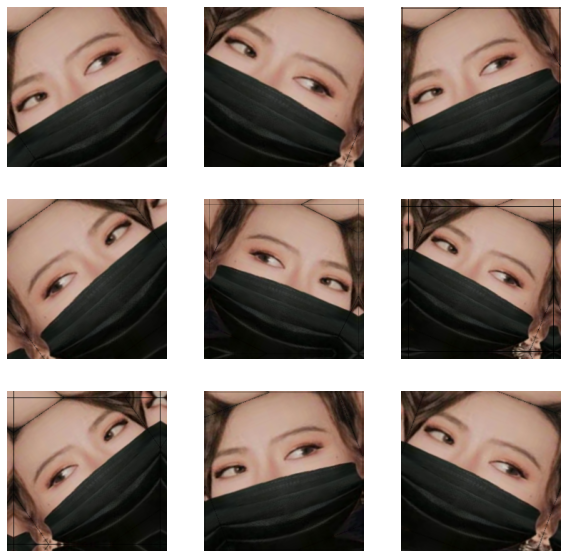
\includegraphics[width=7cm]{augmentation.png}
% \end{center}


% \subsection{Dimensionality reduction}
% \begin{center}
%   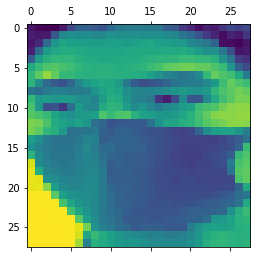
\includegraphics[width=4cm]{pca.png}
% \end{center}

% It can be seen that the picture contains many similar pixels, so referring to the idea of face recognition, we can perform appropriate dimensionality reduction processing through principal component analysis.\\
% \textbf{sklearn.decomposition.PCA} is used here.
% \begin{lstlisting}
% n_components = 15
% pca = PCA(
%   n_components=n_components,
%   svd_solver='randomized',
%   whiten=True
% ).fit(X_train)
% eigenfaces = pca.components_.reshape(
%   (n_components, img_height, img_width)
% )
% X_train_pca = pca.transform(X_train)
% X_test_pca = pca.transform(X_test)
% \end{lstlisting}
% Obviously, after extracting the first 15 main features, we can still clearly distinguish whether people are wearing masks.

% \begin{center}
%   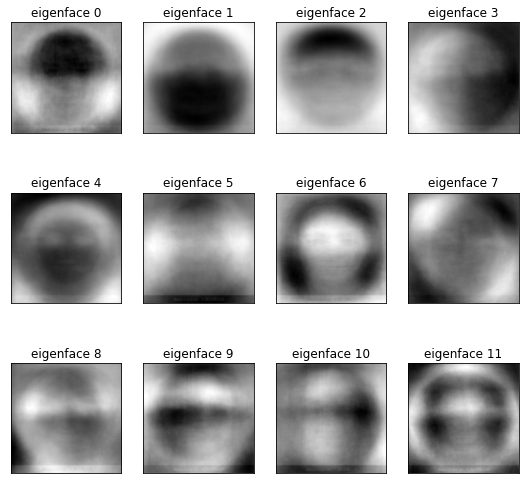
\includegraphics[width=10cm]{eigenfaces.png}
% \end{center}

% \subsection{Classification algorithms}


% \subsubsection{Support Vector Machines}
% I chose C-Support Vector Classification(SVC) with Radial basis function kernel(RBF). Use GridSearchCV to find the optimal SVC parameters C and gamma.
% \textbf{sklearn.model\_selection.GridSearchCV} and \textbf{sklearn.svm.SVC} is used here.
% \begin{lstlisting}
% param_grid = {
%     'C': [1e3, 5e3, 1e4, 5e4, 1e5],
%     'gamma': [0.0001, 0.0005, 0.001, 0.005, 0.01, 0.1]
% }
% SVM = GridSearchCV(
%     SVC(kernel='rbf',
%         class_weight='balanced',
%         probability = True,
%         verbose = True
%         ),
%     param_grid,
%     verbose=10,
%     n_jobs=-1
% )
% SVM = SVM.fit(X_train_pca, y_train)
% print(SVM.best_estimator_)
% \end{lstlisting}

% \subsubsection{Nearest Neighbors}
% For the n\_components, consider the nearest neighbor classifier.

% \subsubsection{Decision Trees}

% \subsubsection{Bayesian Learning}

% \subsubsection{Logistic Regression}


% \section{Results}


% \section{Conclusions and Future Work}


% \section{References}

% \end{document} 
































